\chapter{Lecture 1: New Revolutions in Particle Physics: Standard Model}

These notes follow Leonard Susskind's first lecture in \emph{Particle Physics 2: Standard Model}, with curation by LazyingArt LLC. The lecture begins by delaying, once again, the promised particle list. That delay is not a digression. We already have two sides of the modern picture, particles and fields; before the catalogue can begin in earnest, we need the third side as well, namely force. The lecture therefore unfolds in a very definite order: first the field-language account of force, then the exchange-language account, and only then the first entries of the particle table.

\section{Particles, Fields, and the Missing Third Leg}

By this point in the course we have already built a good deal of machinery. We have fields and their quanta, wave equations and action principles, and the broad kinematic properties of particles: energy, momentum, spin, and the boson-fermion distinction. Fermions resist occupancy of the same state; bosons do not, and may pile up coherently into one state. We also know that products of fields in a Lagrangian encode processes, or vertices, in which particles come in and particles go out.

But something is still missing. Before we start naming the particles one by one, or rather group by group, the lecture insists that we complete a triangle of ideas:
\begin{itemize}
\item particles,
\item fields for which those particles are quanta,
\item forces associated with exchange processes involving those same quanta.
\end{itemize}

There is also a warning here, and it is worth preserving. The distinction between elementary and composite particles is not settled at the outset. We postpone it. For now we imagine that there are fundamental fields and that their quanta are elementary particles. The missing issue is different: if every field corresponds to a particle, and if every familiar field gives rise to a force, then there must also be a way to think about force directly in particle language.

That is the theme of the lecture. We are not going to be satisfied with Coulomb's law as a memorized formula. We want to see where a force comes from in the field description, and then see how the same phenomenon is retold when the field is regarded as a collection of quanta.

\section{Force from Field Energy in Classical Electrodynamics}

Susskind first closes the triangle in the classical language. Suppose we place two charges in space and ask for the force between them. One answer is to quote the inverse-square law. The lecture chooses a better answer: ask what the charges do to space.

They create electric fields. If the first charge produces \(\mathbf{E}_1\) and the second produces \(\mathbf{E}_2\), then the total field is
\begin{equation}
\mathbf{E}=\mathbf{E}_1+\mathbf{E}_2.
\end{equation}
The transcript here is garbled in the details of a temporary charge-rescaled notation, so we keep only the stable mathematical core. The field energy is obtained schematically by squaring the electric field and integrating over space:
\begin{equation}
U_{\text{field}}\propto \int d^3x\,\mathbf{E}^2.
\end{equation}
Substituting the sum of the two fields gives
\begin{align}
U_{\text{field}}
&\propto \int d^3x\,(\mathbf{E}_1+\mathbf{E}_2)^2 \\
&\propto \int d^3x\,\bigl(\mathbf{E}_1^2+\mathbf{E}_2^2+2\,\mathbf{E}_1\!\cdot\!\mathbf{E}_2\bigr).
\end{align}

Now the lecture pauses and reads this expansion term by term. The first term is the self-energy of particle \(1\). The second is the self-energy of particle \(2\). Each is already part of the energy, hence the mass, of the corresponding isolated particle. Each is position-independent. For the present purpose, we set them aside.

The cross-term is different. It is not the energy of either particle separately. It exists only because both are present. If the charges are extremely far apart, the two Coulomb fields scarcely overlap and the integral is negligible. If they are brought closer, the overlap grows, and so does the new contribution. Thus the natural interaction energy is
\begin{equation}
U_{\text{int}}(r)\propto \int d^3x\,\mathbf{E}_1\!\cdot\!\mathbf{E}_2.
\end{equation}
The force is then read from the \(r\)-dependence of this interaction energy:
\begin{equation}
F(r)=-\frac{dU_{\text{int}}}{dr}.
\end{equation}
If one performs the full calculation, one recovers the usual Coulomb behavior,
\begin{equation}
F_{\text{Coulomb}}(r)\propto \frac{q_1q_2}{r^2}.
\end{equation}

This is the lecture's first important payoff. The force law is now understood as coming from the portion of the field energy that depends on the relative arrangement of the two charges. One could say it this way: bring the charges together, the field in between them is distorted, and that distortion carries energy. The force is the derivative of that energy.

But if fields are nothing but collections of quanta, then this cannot be the end of the story. There must also be a particle-language account of the same force.

\section{Molecular Exchange: Two Protons and One Electron}

Before returning to electrodynamics in that second language, the lecture takes a detour to a system where the exchange picture is easier to see. Consider two protons and one electron. This is not chosen because it is the same as electrodynamics. It is chosen because the quantum mechanics is more intuitive.

If one proton is present and the other is taken very far away, the electron occupies the hydrogenic ground state centered on the first proton. The board first records this simply as a localized hump.

\begin{figure}[h]
\centering

\includegraphics[width=0.72\textwidth]{lecture_01_figure_02.png}

\medskip

\begin{tikzpicture}[scale=0.95]
\draw (-0.2,0) -- (6.4,0);
\fill (1.3,0) circle (2pt);
\draw[smooth] plot coordinates {(0.1,0.15) (0.8,1.15) (1.5,1.75) (2.2,1.1) (3.0,0.35) (3.8,0.12)};
\node at (1.3,-0.35) {$p$};
\node at (2.7,1.55) {$\psi_1(x)$};
\end{tikzpicture}
\caption{Single hydrogenic wave-function sketch. The frame documents the board layout; the TikZ curve is a cleaned schematic reading rather than a literal transcription of notation.}
\end{figure}

The faint point label beneath the chalk mark looks like a handwritten \(P\), but it is too uncertain to be used as reliable notation. What matters is the shape: a bound-state profile localized near one force center.

Now place a second proton at finite but large separation. By symmetry there is a second localized state of the same energy, centered near the right proton.

\begin{figure}[h]
\centering

\includegraphics[width=0.78\textwidth]{lecture_01_figure_03.png}

\medskip

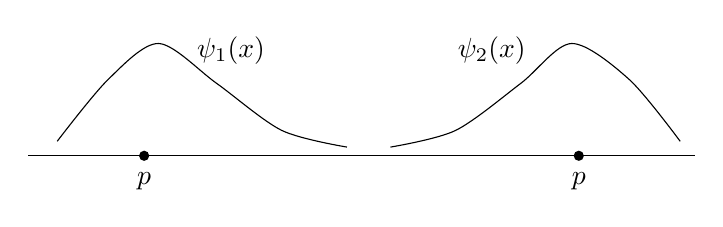
\begin{tikzpicture}[scale=0.92]
\draw (-0.2,0) -- (9.0,0);
\fill (1.4,0) circle (2pt);
\fill (7.4,0) circle (2pt);
\draw[smooth] plot coordinates {(0.2,0.2) (0.9,1.05) (1.6,1.55) (2.4,1.0) (3.3,0.35) (4.2,0.12)};
\draw[smooth] plot coordinates {(4.8,0.12) (5.7,0.35) (6.6,1.0) (7.3,1.55) (8.1,1.05) (8.8,0.2)};
\node at (1.4,-0.35) {$p$};
\node at (7.4,-0.35) {$p$};
\node at (2.6,1.45) {$\psi_1(x)$};
\node at (6.2,1.45) {$\psi_2(x)$};
\end{tikzpicture}
\caption{Two localized electron wave functions. The lecture now moves from these two one-center states to an equilibrium superposition.}
\end{figure}

At infinite separation the two states are degenerate. The electron may be localized near the left proton or near the right proton, and the energy is the same.

\subsection{Question \& Answer}

\paragraph{Question.} Why is the two-proton system not exactly degenerate once the separation is finite?

\paragraph{Answer.} Because once the protons are not infinitely far apart, processes become possible that were impossible before. In particular, the electron can tunnel from one center to the other. The lecture first describes this qualitatively, but the minimal mathematical reconstruction is a two-state Hamiltonian. If \(|L\rangle\) and \(|R\rangle\) denote the left- and right-localized states, then finite separation introduces off-diagonal matrix elements:
\begin{align}
H|L\rangle &= E_0 |L\rangle - t |R\rangle,\\
H|R\rangle &= E_0 |R\rangle - t |L\rangle,
\end{align}
with \(t>0\) a tunneling amplitude.

The eigenstates are therefore the symmetric and antisymmetric combinations
\begin{align}
|+\rangle &= \frac{|L\rangle+|R\rangle}{\sqrt2},
&
E_+ &= E_0-t,
\\
|-\rangle &= \frac{|L\rangle-|R\rangle}{\sqrt2},
&
E_- &= E_0+t.
\end{align}
Translated back into wave functions, the lower equilibrium state is approximately
\begin{equation}
\psi_+(x)\approx \frac{\psi_1(x)+\psi_2(x)}{\sqrt2}.
\end{equation}

The word ``approximately'' matters. The lecture is explicit that the true equilibrium wave function is not \emph{exactly} the naive sum. In the overlap region between the two wells it is slightly different. The accepted frame does not settle the exact contour there, and in any case Susskind himself says he did not draw it very well. But the physical point is stable: once tunneling is allowed, the true equilibrium state has lower energy than the two isolated one-center states.

The lecture also says what one should not do. One should not picture this as a literal observed trajectory, with the electron watched in transit. As in the rest of quantum mechanics, trying to watch the tunneling ruins the phenomenon. The exchange picture is a way of describing the state, not a classical movie of a particle moving through space.

\section{From Lowered Energy to an Effective Force}

Now the lecture shifts, very deliberately, from the shape of the state to the shape of the energy. At large proton separation the electron energy is just the familiar one-center ground-state energy. At smaller separation, once tunneling and superposition are allowed, the equilibrium energy is slightly lower. Therefore the energy of the whole two-proton one-electron system becomes a function of the proton separation \(r\).

This is the exact point at which the molecular example reconnects with the field-theory example. We may regard that separation-dependent energy as an effective potential \(V(r)\). The board then adds the second, lower sketch: a qualitative graph of energy against separation.

\begin{figure}[h]
\centering

\includegraphics[width=0.78\textwidth]{lecture_01_figure_04.png}

\medskip

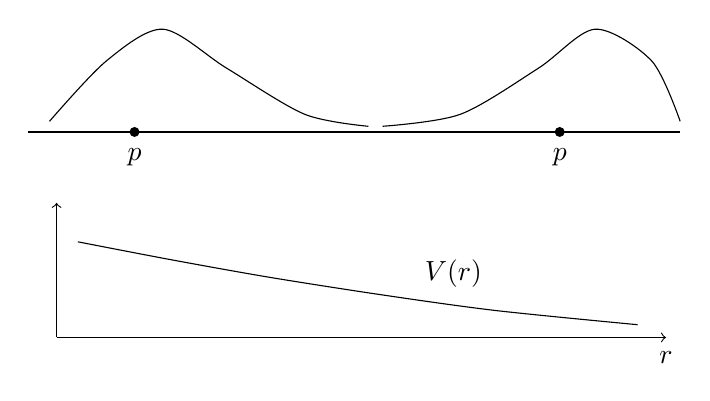
\begin{tikzpicture}[scale=0.9]
\draw (-0.2,3.0) -- (9.0,3.0);
\fill (1.3,3.0) circle (2pt);
\fill (7.3,3.0) circle (2pt);
\draw[smooth] plot coordinates {(0.1,3.15) (0.9,4.0) (1.7,4.45) (2.6,3.9) (3.7,3.25) (4.6,3.08)};
\draw[smooth] plot coordinates {(4.8,3.08) (5.9,3.25) (7.0,3.9) (7.8,4.45) (8.6,4.0) (9.0,3.15)};
\node at (1.3,2.65) {$p$};
\node at (7.3,2.65) {$p$};

\draw[->] (0.2,0.1) -- (0.2,2.0);
\draw[->] (0.2,0.1) -- (8.8,0.1);
\draw[smooth] plot coordinates {(0.5,1.45) (1.8,1.2) (3.2,0.95) (4.8,0.7) (6.4,0.48) (8.4,0.28)};
\node at (5.8,1.0) {$V(r)$};
\node at (8.8,-0.18) {$r$};
\end{tikzpicture}
\caption{Wave-function overlap and effective proton potential. The board image supports the two-level layout; the label \(V(r)\) is a cleaned choice, since the frame itself does not fix whether the intended ordinate was \(E\) or \(V\).}
\end{figure}

The force is now read from the energy gradient:
\begin{equation}
F(r)=-\frac{dV}{dr}.
\end{equation}
The lecture phrases it in plain language: force pushes toward decreased energy. If the energy drops as the protons move together, then the system experiences an effective attraction.

This is the molecular version of the same logic we saw earlier for classical fields. In one case the energy change comes from the overlap of two electric fields. In the other it comes from the lowering of the quantum-mechanical equilibrium energy in a two-center problem. In both cases, force comes from a configuration-dependent energy.

Several audience questions sharpen the intended picture, and they are worth preserving because otherwise the discussion becomes too loose.

\paragraph{What the picture is not.}
\begin{itemize}
\item It is not mainly a screening story. The essential point is not that the electron merely reduces the proton charge seen by the other proton.
\item It is not a third independent force in addition to the familiar ones. Rather, the Schr\"odinger problem in the presence of two force centers has a lower equilibrium energy than the sum of two isolated one-center problems.
\item It is not best described as ordinary two-particle entanglement. The lecture says more pointedly that the relevant structure is the presence of off-diagonal elements in the Hamiltonian.
\item It is not a literal watched trajectory. The worldline picture is schematic, useful for intuition and dangerous if taken too seriously.
\end{itemize}

The lecture also emphasizes a limitation. In the one-electron system the two protons still carry net positive charge, so Coulomb repulsion remains. The exchange attraction is short-ranged; the electrostatic repulsion is longer-ranged. Thus attraction does not automatically mean stable binding at all separations. In a neutral two-electron system, by contrast, the long-range Coulomb piece is much less dominant, and the same exchange mechanism shows up more cleanly as ordinary molecular binding.

The exchange picture can nevertheless be drawn, and the lecture does draw it in words.

\begin{figure}[h]
\centering
\begin{tikzpicture}[scale=1.0]
\draw (0,0) -- (0,4.4);
\draw (4.8,0) -- (4.8,4.4);
\draw (0,0.9) .. controls (1.6,1.7) and (3.2,1.7) .. (4.8,2.5);
\draw (4.8,2.9) .. controls (3.2,2.1) and (1.6,2.1) .. (0,3.9);
\node at (0,-0.35) {$p$};
\node at (4.8,-0.35) {$p$};
\node at (2.35,1.55) {$e^-$};
\node at (2.35,2.55) {$e^-$};
\end{tikzpicture}
\caption{Transcript-backed schematic of electron exchange between two proton worldlines. This is an explanatory reconstruction of the lecture's picture, not a direct board transcription.}
\end{figure}

\section{Photon Exchange and the First Entries of the Table}

Now that the exchange picture has been made visible in a molecular setting, the lecture returns to electrodynamics. Can the Coulomb force be told in the same language? Yes. A charged particle interacts with the electromagnetic field, and the quanta of that field are photons. Classically one solves for an electric field around the charge. Quantum mechanically one thinks instead in terms of emission and absorption of photons.

The lecture makes this more concrete. A physical charged particle is not just a bare charge. It is a quantum-mechanical superposition of states containing no photons, one emitted photon, two photons, and so on, with photons continually emitted and reabsorbed. If another charged particle is nearby, then a photon emitted by one may be absorbed by the other. That shared-photon process changes the energy of the two-particle system away from the simple sum of two isolated energies. That energy shift is the Coulomb interaction in particle language.

This is the place where Susskind explicitly closes the triangle. Particles, fields, and forces are now in one-to-one-to-one correspondence. When people say there are only four forces in nature, the lecture pushes back. In the exchange sense, every exchangeable quantum can mediate a force in some appropriate context. Electrons do so in molecular physics. Photons do so in electrodynamics.

Only after this bridge has been built does the lecture finally allow itself to start the table of particles. And even here the style matters. He does not want to dump the whole Standard Model on the board at once. Better to proceed in small groups, because the full thing is, as he says, a monstrosity.

The accepted frame should remain visible, because it captures exactly that switch in board logic.

\begin{figure}[h]
\centering

\includegraphics[width=0.7\textwidth]{lecture_01_figure_05.png}
\caption{Photon symbol and vector-potential notation. The crop securely shows the photon row and the entries \(\gamma\) and \(A\).}
\end{figure}

The board evidence supports the secure identification
\begin{equation}
\gamma \leftrightarrow A.
\end{equation}
The lecture then explains in words that \(A\) is the electromagnetic vector potential. In a later, more covariant notation one would often write \(A_\mu\), but the board itself only visibly shows \(A\), so that is the notation we keep at first pass.

The table columns are introduced in a specific order: name, symbol, type, charge, baryon number, and mass. Here ``type'' means simply boson or fermion. The first secure row is the photon row; the next row, for the electron and positron, comes from the transcript rather than from the crop itself.

\begin{table}[h]
\centering
\begin{tabular}{lllllll}
Name & Symbol & Field & Type & \(Q\) & \(B\) & Mass \\
Photon & \(\gamma\) & \(A\) & boson & \(0\) & \(0\) & \(0\) \\
Electron/positron & \(e^\pm\) & \(\psi_e\) & fermion & \(\mp 1\) & \(0\) & \(0.51\,\mathrm{MeV}\)
\end{tabular}
\caption{A cleaned continuation of the lecture's first table entries. Only the photon row is directly visible in the accepted crop; the electron row is added from the transcript.}
\end{table}

Here the lecture slows down again for units and conventions. Electric charge is measured in units of the electron charge. Thus we simply write
\begin{equation}
Q(e^-)=-1,\qquad Q(e^+)=+1.
\end{equation}
Likewise mass is measured in energy units, since \(E=mc^2\). The historically natural unit is the electron volt, and in particle physics we quickly move to MeV and GeV. The electron mass is
\begin{equation}
m_e \approx 0.51\,\mathrm{MeV}.
\end{equation}
The lecture also remarks that it is conventional to speak of the electron as the particle and the positron as its antiparticle, though the relation is actually mutual; choosing which one to call ``the particle'' is a convention of language.

The elementary QED process is then introduced: one electron in, one electron out, one photon attached. By rearranging the legs of that one vertex one reads the same diagram as emission, absorption, or positron emission. At the lecture's level the interaction term is described schematically as a product of one electron field in, one electron field out, and one photon field:
\begin{equation}
\mathcal{L}_{\mathrm{int}}\sim e\,\psi_e^\dagger \psi_e A.
\end{equation}
This is intentionally schematic. A more modern covariant form would refine both the spinor structure and the photon field notation, but the lecture's real point is simpler:
\begin{equation}
\mathcal{A}(e\to e+\gamma)\propto e,
\qquad
P(e\to e+\gamma)\propto e^2.
\end{equation}

A schematic vertex is therefore useful.

\begin{figure}[h]
\centering
\begin{tikzpicture}[scale=1.0]
\fill (0,0) circle (1.5pt);
\draw (-1.6,-1.2) -- (0,0) -- (1.6,-1.2);
\draw (0,0) -- (0,1.8);
\node at (-1.8,-1.4) {$e^-$};
\node at (1.8,-1.4) {$e^-$};
\node at (0.35,1.95) {$\gamma$};
\end{tikzpicture}
\caption{Schematic QED vertex: one electron in, one electron out, one photon attached. By crossing the legs, the lecture reads the same vertex in several ways.}
\end{figure}

And the force between charges is the many-body consequence of such elementary emission and absorption events:

\begin{figure}[h]
\centering
\begin{tikzpicture}[scale=1.0]
\draw (0,0) -- (0,4.0);
\draw (4.8,0) -- (4.8,4.0);
\draw (0,2.0) -- (4.8,2.0);
\node at (0,-0.35) {$e^-$};
\node at (4.8,-0.35) {$e^-$};
\node at (2.4,2.3) {$\gamma$};
\end{tikzpicture}
\caption{Transcript-backed schematic of photon exchange. In the lecture this is the quantum-field-theoretic retelling of the Coulomb interaction.}
\end{figure}

At this point the opening promise can finally be kept. We are ready to begin naming the players.

\section{Quarks, Baryon Number, and the Puzzle of Families}

The next move is historically important. In an earlier era one might have gone directly from electrons and photons to protons and neutrons. The lecture instead says: no, modern particle physics places quarks first. Protons and neutrons are to be understood, at least naively, as composites of quarks.

There are six quark flavors,
\begin{equation}
u,\ d,\ s,\ c,\ b,\ t,
\end{equation}
and the lecture is almost amused by the naming conventions. Up and down are not really up and down. Strange is not stranger than the others. Charm, bottom, and top are historical accidents. The names are not the structure.

The structure comes in two parts. First, all quarks are fermions. Second, their charges repeat in pairs:
\begin{equation}
Q(u)=Q(c)=Q(t)=+\frac23,
\qquad
Q(d)=Q(s)=Q(b)=-\frac13.
\end{equation}
Thus the trio \((d,u)\), \((s,c)\), and \((b,t)\) exhibits a pattern of replicated charge assignments. But the masses do not remotely repeat:
\begin{align}
m_u &\sim 5\,\mathrm{MeV},
&
m_d &\sim 10\,\mathrm{MeV},
\\
m_s &\sim 100\,\mathrm{MeV},
&
m_c &\sim 10^3\,\mathrm{MeV},
\\
m_b &\sim 5\,\mathrm{GeV},
&
m_t &\sim 170\,\mathrm{GeV}.
\end{align}
So the lecture presses on a tension that is central to the Standard Model. The quarks are in one sense copies of one another; in another sense their mass scales wander across several orders of magnitude. That repetition of families without any satisfying explanation is one of the deep puzzles of the subject.

The lecture also restores some phenomenological perspective. Of the six quark flavors, only \(u\) and \(d\) appear abundantly in ordinary matter. The heavier ones decay down the chain. So low-energy physics is dominated by the first family, while the others are present as heavier echoes.

\subsection{Question \& Answer}

\paragraph{Question.} Why does a quark carry baryon number \(1/3\), and can baryon number be violated?

\paragraph{Answer.} Baryon number is introduced operationally, not metaphysically. One first counts protons and neutrons. By convention,
\begin{equation}
B(p)=1,\qquad B(n)=1.
\end{equation}
That normalization could have been chosen differently; the lecture explicitly remarks that one could have called it \(2\), or \(7\), or \(\pi\), as long as it scaled consistently. Once the proton is recognized as a three-quark object, however, consistency forces
\begin{equation}
B(q)=\frac13,
\qquad
B(\bar q)=-\frac13.
\end{equation}
So the factor \(1/3\) is not a new mystery. It is the inherited normalization of a bookkeeping convention.

The sharper question is whether baryon number is exact. Empirically it is conserved to extremely high precision, but the lecture refuses to promote that fact into an exact law. A decay such as
\begin{equation}
p\to e^+ + \gamma
\end{equation}
would conserve electric charge and still violate baryon number. No such process has been observed; the proton lifetime must be at least of order \(10^{33}\) to \(10^{34}\) years. But that does not amount to a proof that baryon number is absolute. The lecture leaves the question open.

A further caution is also preserved. Quarks are not observed as isolated free particles. One can certainly detect evidence of quarks, but not a lone quark sitting in isolation waiting to be measured.

\section{From Quarks to Hadrons: Nucleons, Strange Baryons, and Mesons}

Once the quark charges are known, familiar hadrons can be rebuilt. The first examples are the neutron and proton:
\begin{equation}
n=ddu,
\qquad
p=uud.
\end{equation}

\paragraph{Worked example.} The lecture explicitly checks the charges:
\begin{align}
Q(n) &= Q(d)+Q(d)+Q(u)
= -\frac13-\frac13+\frac23
=0,\\
Q(p) &= Q(u)+Q(u)+Q(d)
= \frac23+\frac23-\frac13
=1.
\end{align}

Now comes a characteristic Susskind move. Forget photons for a moment. If we ignore electromagnetism and focus only on the quark content, then proton and neutron look almost like the same object with \(u\) and \(d\) interchanged. This suggests a near-symmetry. It is not exact, because \(u\) and \(d\) do not have exactly the same masses.

That near-symmetry is good enough to tell us the sign of the proton-neutron mass difference. Since \(m_d>m_u\), the neutron, which contains more down quarks, should be slightly heavier. And it is. Electromagnetic self-energy by itself would push the other way and make the proton heavier, because the proton is charged. The observed ordering therefore tells us that the \(d-u\) mass difference wins over the electromagnetic correction.

\begin{remark}
The lecture also points out the famous mismatch in the nucleon mass budget. The quark masses add up to only a few MeV, whereas the proton and neutron masses are around \(940\,\mathrm{MeV}\). The missing contribution is not mysterious ``stuff'' hidden in the nucleon; it is energy carried by the gluonic and binding dynamics. The lecture's summary is blunt: masses do not simply add relativistically for bound systems.
\end{remark}

The same constituent logic produces strange baryons. Since \(s\) and \(d\) have the same electric charge, one may replace a down quark by a strange quark without changing the charge pattern:
\begin{equation}
uds,\qquad uss,\qquad uus.
\end{equation}
These are analogs of the ordinary nucleons, but heavier, and therefore unstable. They decay down to lighter baryons plus other particles. The lecture is not yet trying to classify the decays in detail; it is simply establishing that the strange quark may be inserted into the same three-quark structures.

At this point the lecture inserts a useful rule of thumb. Why do three quarks bind into baryons? Why not two quarks? In the early days of quark theory this was a genuine puzzle. At the level of this lecture no full derivation is offered. Instead one adopts the empirical rule that the bound states one actually encounters carry charges that are integer multiples of the electron charge. Baryons do so with three quarks; mesons do so with quark-antiquark pairs. The lecture explicitly treats this as a working rule before deeper explanations are taken up.

Mesons are therefore introduced next as \(q\bar q\) composites. Their baryon number vanishes:
\begin{equation}
B(q\bar q)=\frac13-\frac13=0.
\end{equation}
The first mesons to discuss are the ones built only from \(u\) and \(d\), because those are the light quarks: they are abundant, comparatively stable, and cheap to produce.

The natural flavor basis is
\begin{equation}
|\bar u d\rangle,\qquad |u\bar d\rangle,\qquad |\bar u u\rangle,\qquad |\bar d d\rangle.
\end{equation}
The charged states are immediate:
\begin{equation}
|\pi^-\rangle=|\bar u d\rangle,
\qquad
|\pi^+\rangle=|u\bar d\rangle.
\end{equation}

\subsection{Question \& Answer}

\paragraph{Question.} Why are the neutral meson states written as superpositions rather than as separate \(\bar u u\) and \(\bar d d\) particles?

\paragraph{Answer.} Because at this point the lecture is explicitly doing quantum mechanics. The states \(|\bar u u\rangle\) and \(|\bar d d\rangle\) are a basis, not automatically the physical particles. One may superpose them, and in fact the lecture says that neither one by itself corresponds to a distinct particle. The two orthogonal combinations are
\begin{align}
|\pi^0\rangle &\approx \frac{|\bar u u\rangle-|\bar d d\rangle}{\sqrt2},\\
|\eta\rangle &\approx \frac{|\bar u u\rangle+|\bar d d\rangle}{\sqrt2}.
\end{align}

This is also the lecture's first glimpse of isospin. Upness and downness are treated as a two-state internal degree of freedom, analogous in a loose way to spin up and spin down. In that language the neutral combinations are not arbitrary. They are the natural sum and difference states in the two-dimensional flavor space.

The pion triplet \(\pi^+,\pi^0,\pi^-\) goes together because the three masses are close. In the limit \(m_u=m_d\), they would be even closer, ideally degenerate. The orthogonal neutral state is the \(\eta\), which behaves similarly in many respects but sits higher in mass:
\begin{equation}
m_\pi \approx 140\,\mathrm{MeV},
\qquad
m_\eta \approx 500\,\mathrm{MeV}.
\end{equation}
The lecture treats the anomalous heaviness of the \(\eta\) as an important but more complicated story, not to be unpacked in this first chapter.

A further empirical remark from the lecture is worth keeping: the pions are comparatively long-lived because they do not decay by the strong interaction. Their decays proceed only through weaker channels.

Finally, once the strange quark is admitted, one obtains the strange mesons or \(K\)-mesons by replacing \(d\) or \(\bar d\) with \(s\) or \(\bar s\). The flavor states are
\begin{equation}
\bar u s,\qquad u\bar s,\qquad \bar d s,\qquad d\bar s.
\end{equation}
Their charge assignments are
\begin{align}
Q(\bar u s) &=-1,
&
Q(u\bar s) &=+1,
\\
Q(\bar d s) &=0,
&
Q(d\bar s) &=0.
\end{align}
So there are two charged \(K\)-mesons and two neutral ones.

Counting all light \(u,d,s\) quarks and antiquarks gives
\begin{equation}
3\times 3 = 9
\end{equation}
light flavor combinations in all. The lecture stops there, deliberately before complete classification. The first map of the territory has been drawn, but only in outline. That is exactly the right stopping point for Lecture 1.

\section{Summary}

The lecture begins by postponing the particle list and ends by justifying that postponement. We first see, in classical electrodynamics, that force can be read from the part of the field energy that depends on configuration. We then see the same idea retold in a different language through molecular exchange: two centers, tunneling, superposition, lowered energy, and therefore attraction.

Only after that bridge is built does the lecture shift into catalogue mode. The photon and its field \(A\), the electron and its field \(\psi_e\), the QED vertex, then quarks, baryon number, replicated families, nucleons, strange baryons, and neutral meson superpositions. The Standard Model is not presented as a finished elegant structure. It is presented, more honestly, as a partly organized and partly mysterious collection of particles whose patterns are visible long before their deepest explanation is in hand.

That is the right tone for the beginning of the subject. The lecture does not merely list what exists. It shows us how the concepts fit together well enough that the list can begin to mean something.